\documentclass[a4paper]{report}
\usepackage[utf8]{inputenc}
\usepackage[T1]{fontenc}
\usepackage{RJournal}
\usepackage{amsmath,amssymb,array}
\usepackage{booktabs}


% tightlist command for lists without linebreak
\providecommand{\tightlist}{%
  \setlength{\itemsep}{0pt}\setlength{\parskip}{0pt}}

\usepackage{longtable}

% Always define CSL refs as bib entries are contained in separate doc
% Pandoc citation processing
\newlength{\cslhangindent}
\setlength{\cslhangindent}{1.5em}
\newlength{\csllabelwidth}
\setlength{\csllabelwidth}{3em}
\newlength{\cslentryspacingunit} % times entry-spacing
\setlength{\cslentryspacingunit}{\parskip}
% for Pandoc 2.8 to 2.10.1
\newenvironment{cslreferences}%
  {}%
  {\par}
% For Pandoc 2.11+
\newenvironment{CSLReferences}[2] % #1 hanging-ident, #2 entry spacing
 {% don't indent paragraphs
  \setlength{\parindent}{0pt}
  % turn on hanging indent if param 1 is 1
  \ifodd #1
  \let\oldpar\par
  \def\par{\hangindent=\cslhangindent\oldpar}
  \fi
  % set entry spacing
  \setlength{\parskip}{#2\cslentryspacingunit}
 }%
 {}
\usepackage{calc}
\newcommand{\CSLBlock}[1]{#1\hfill\break}
\newcommand{\CSLLeftMargin}[1]{\parbox[t]{\csllabelwidth}{#1}}
\newcommand{\CSLRightInline}[1]{\parbox[t]{\linewidth - \csllabelwidth}{#1}\break}
\newcommand{\CSLIndent}[1]{\hspace{\cslhangindent}#1}


\usepackage{float} \floatplacement{figure}{H}

\begin{document}


%% do not edit, for illustration only
\sectionhead{Contributed research article}
\volume{XX}
\volnumber{YY}
\year{20ZZ}
\month{AAAA}

\begin{article}
  % !TeX root = RJwrapper.tex
\title{sugarglider: Create glyphmaps of spatio-temporal data}


\author{by Maliny Po and Dianne Cook}

\maketitle

\abstract{%
(An abstract of less than 150 words.)
}

\hypertarget{introduction}{%
\section{Introduction}\label{introduction}}

\begin{verbatim}
Note: use similar terminology as cubble & glyph-maps. Add a quick start (quick guide on how to use the sugarglider package)
\end{verbatim}

\hypertarget{literature-review}{%
\section{Literature Review}\label{literature-review}}

\hypertarget{glyph-maps}{%
\subsubsection{Glyph Maps}\label{glyph-maps}}

\begin{itemize}
\item
  Glyph maps are a specific type of multivariate glyph plots where each spatial location is represented by a glyph that encapsulates data measured over time at that location. As detailed in \href{https://vita.had.co.nz/papers/glyph-maps.pdf}{Hadley Wickham's} paper, glyph maps are particularly effective for uncovering both local and global structures, emphasizing temporal relationships within the data. These maps utilize small glyphs or icons to represent multiple data values at each location, extending the concept of glyphs which are traditionally used to display multivariate data.
\item
  Challenges with Faceted Maps and Spatio-Temporal Animations: While faceted maps and spatio-temporal animations are useful for highlighting spatial patterns, they often fall short in adequately showcasing temporal trends. To overcome this, a transformation technique is employed which utilizes principles of linear algebra to convert temporal coordinates (minor coordinates) into spatial coordinates (major coordinates). This transformation is implemented in packages such as \href{https://cran.r-project.org/web/packages/GGally/GGally.pdf}{GGally} and \href{https://www.jstatsoft.org/article/view/v110i07}{cubble}, facilitating a more integrated approach to spatio-temporal data visualization.
\item
  The R package \href{https://www.jstatsoft.org/article/view/v110i07}{cubble} introduces an innovative cubble class designed to efficiently organize spatial and temporal variables. This dual structure allows for separate or combined manipulation of these variables while maintaining synchronization. A spatial cubble object is constructed from distinct spatial and temporal tables through the function make\_cubble(), requiring the specification of three attributes: key, index, and coords. This functionality not only simplifies the data wrangling process but also enhances the analytical capabilities when dealing with complex datasets.
\end{itemize}

\hypertarget{extending-ggplot2-with-ggproto}{%
\subsubsection{Extending ggplot2 with ggproto}\label{extending-ggplot2-with-ggproto}}

\begin{verbatim}
 Diversify your resources a bit :((
\end{verbatim}

\begin{itemize}
\tightlist
\item
  Elegant Graphics for Data Analysis: The architecture of ggplot2 is fundamentally based on the ggproto system of object-oriented programming. Initially, ggplot2 utilized the proto system, developed by Grothendieck, Kates, and Petzoldt in 2016, for object-oriented tasks. This system, described in detail in the \href{https://cran.r-project.org/web/packages/proto/proto.pdf}{Proto package documentation},
  outlines that proto is an S3 subclass of the R environment class, implying single inheritance and mutable state characteristic of all environments. Proto objects are created and modified using the proto function which sets the parent environment, evaluates expressions, and handles lazy evaluation of arguments.
\end{itemize}

However, as the need for an official extension mechanism in ggplot2 grew, the limitations of the proto system became apparent, leading to the adoption of ggproto. This transition is well-documented in Hadley Wickham's book, \href{https://ggplot2-book.org/}{ggplot2: Elegant Graphics for Data Analysis}, which also introduces how to utilize ggproto objects to extend ggplot2 functionalities.

The creation of a new ggproto object is facilitated by the ggproto() function, which requires the name of the new class and an existing ggproto object from which it will inherit. For instance, to introduce a new statistical transformation, one might create a ggproto that inherits from \texttt{Stat} and \texttt{Geom.} However, merely creating a ggproto object does not make it accessible or useful to the end user.

(Example from ggplot2-book.org)

\begin{verbatim}
NewObject <- ggproto(
  `_class` = NULL, 
  `_inherits` = NULL
)
\end{verbatim}

To bridge this gap, the creation of a layer function is necessary. An example is the \texttt{new\_stat()} function, which follows a consistent format: setting defaults in the function arguments, and calling layer(), which handles the distribution of these arguments into either geom parameters, stat parameters, or aesthetics. This function exemplifies the methodology to create functional and user-accessible components in ggplot2.

(Example from ggplot2-book.org)

\begin{verbatim}
new_stat <- function(mapping = NULL, data = NULL, 
                       geom = "geometry", position = "identity", 
                       na.rm = FALSE, show.legend = NA, 
                       inherit.aes = TRUE, ...) {
  layer(
    stat = NewStat, 
    data = data, 
    mapping = mapping, 
    geom = geom, 
    position = position, 
    show.legend = show.legend, 
    inherit.aes = inherit.aes, 
    params = list(na.rm = na.rm, ...)
  )
}
\end{verbatim}

While developing ggplot2 extensions, it may seem intuitive to encapsulate extensions as new geoms, as they are frequently used by users to add layers to a plot. However, the diversity in ggplot2's capabilities often stems more from the variety in statistical transformations (stats) than merely geometric objects (geoms), suggesting a nuanced approach in designing extensions that effectively enhance the plotting system.

\hypertarget{software}{%
\section{Software}\label{software}}

The \texttt{sugarglider} package extends the capabilities of ggplot2 by introducing functions specifically designed for visualizing seasonal patterns in spatio-temporal data. It includes \texttt{geom\_glyph\_ribbon()} and \texttt{geom\_glyph\_segment()} , which represent measurements recorded over time at specific locations through the use of glyph maps. These functions enable clear depictions of seasonal trends by leveraging the combination of \emph{x\_major} and \emph{y\_major} coordinates.

The package supports the creation of glyph plots using either ribbon or segment geometries. The core functionality is outlined as follows:

\begin{itemize}
\item
  \texttt{geom\_glyph\_ribbon()}: Displays an interval on the y-axis for each \emph{x\_minor} value, with the bounds defined by \emph{ymin\_minor} and \emph{ymax\_minor}. This function draws ribbon geometry using \texttt{geom\_ribbon()} from ggplot2 to draw ribbon geometry, resulting in ribbon glyphs. Each glyph is plotted based on the combination of \emph{x\_major} and \emph{y\_major} coordinates. This functionality is particularly useful for visualizing ranges or uncertainties in the data.
\item
  \texttt{geom\_glyph\_segment()}: Connects \emph{y\_minor} to \emph{yend\_minor} with a straight line using \texttt{geom\_segment()} from ggplot2, resulting in segment glyphs. Each glyph is plotted based on the combination of \emph{x\_major} and \emph{y\_major} coordinates.
\end{itemize}

In addition to these two functions, sugarglider offers several other features that enhance the customization of glyph maps. The \texttt{add\_ref\_box()} function introduces reference boxes that visually frame individual glyphs, helping to define boundaries and distinguish glyphs from each other. The \texttt{add\_ref\_line()} function draws a horizontal midpoint for each glyph, facilitating comparisons across data points. The \texttt{add\_glyph\_legend()} function allows users to display an enlarged version of a randomly chosen glyph in the bottom-left corner of the panel, enabling users to visualize the data range. Lastly, the \texttt{theme\_glyph()} function provides a customized theme for glyph maps, built on top of \texttt{theme\_map()} from \texttt{ggthemes}. It adjusts the plot's appearance, including the legend position, text styles, and background settings, to create a clean, visually consistent layout for glyph visualizations.

\begin{verbatim}
# Ribbon glyph
vic_temp |>
   ggplot(aes(x_major = long,
              y_major = lat,
              x_minor = month,
              ymin_minor = tmin,
              ymax_minor = tmax)) +
  add_glyph_boxes() +
  add_ref_lines() +
  geom_glyph_ribbon() +
  theme_glyph()

# Segment glyph
vic_temp |>
   ggplot(aes(x_major = long,
              y_major = lat,
              x_minor = month,
              y_minor = tmin,
              yend_minor = tmax)) +
  add_glyph_boxes() +
  add_ref_lines() +
  geom_glyph_segment() +
  theme_glyph()
\end{verbatim}

\begin{figure}
\centering
\includegraphics{sugarglider_files/figure-latex/comparisonPlot-1.pdf}
\caption{\label{fig:comparisonPlot}Comparison between ribbon and segment glyph-maps: Glyph boxes and reference lines have been added to frame each glyph and introduce a line that divide each glyph midway, assisting users in making inferences about the plot. Additional coding is required to establish the base map and adjust the width and height of each glyph.}
\end{figure}

The sugarglider package offers a variety of customization options for enhanced visualization flexibility. It includes features such as the \emph{global\_rescale} argument, which allows for choosing between global or individual glyph scaling. Users can also adjust the scaling of minor values within grid cells, as well as the overall width and height of glyphs, ensuring that glyph-map can be finely tuned to meet specific data representation needs. The following section will explore these features in greater detail and provide practical examples that illustrate their application within different visualization contexts.

\hypertarget{aesthetics}{%
\subsubsection{Aesthetics}\label{aesthetics}}

sugarglider provides the same aesthetics for \texttt{geom\_glyph\_ribbon()} and \texttt{geom\_glyph\_segment()} as those available in \texttt{geom\_ribbon()} and \texttt{geom\_segment()} from ggplot2. To include a variable in the glyph plot, it must be specified as an aesthetic. The functions in sugarglider expect spatial coordinates as the major axis and temporal data, along with some measurements, as the minor axis.

To produce glyph-maps, the following aesthetics are required:

\begin{longtable}[]{@{}
  >{\raggedright\arraybackslash}p{(\columnwidth - 2\tabcolsep) * \real{0.2381}}
  >{\raggedright\arraybackslash}p{(\columnwidth - 2\tabcolsep) * \real{0.7619}}@{}}
\toprule\noalign{}
\begin{minipage}[b]{\linewidth}\raggedright
Aesthetics
\end{minipage} & \begin{minipage}[b]{\linewidth}\raggedright
Description
\end{minipage} \\
\midrule\noalign{}
\endhead
\bottomrule\noalign{}
\endlastfoot
\texttt{x\_major},\texttt{y\_major} & Spatial coordinates that define the position of glyphs. \\
\texttt{x\_minor} & Represents temporal data associated with each glyph. \\
\texttt{ymin\_minor}, \texttt{ymax\_minor} & Used by \texttt{geom\_glyph\_ribbon()} to establish the lower and upper bounds of the ribbon geometry within each glyph. \\
\texttt{y\_minor}, \texttt{yend\_minor} & Used by \texttt{geom\_glyph\_segment()} to set the start and end points of the segment geometry within each glyph. \\
\end{longtable}

The functions \texttt{add\_ref\_box()}, \texttt{add\_ref\_line()}, and \texttt{add\_geom\_legend()} are compatible with either \emph{ymin\_minor}, \emph{ymax\_minor}, or \emph{y\_minor}, \emph{yend\_minor}. Additionally, sugarglider introduces several customizable options to further tailor the visual aspects:

\begin{longtable}[]{@{}
  >{\raggedright\arraybackslash}p{(\columnwidth - 4\tabcolsep) * \real{0.2000}}
  >{\raggedright\arraybackslash}p{(\columnwidth - 4\tabcolsep) * \real{0.1600}}
  >{\raggedright\arraybackslash}p{(\columnwidth - 4\tabcolsep) * \real{0.6400}}@{}}
\toprule\noalign{}
\begin{minipage}[b]{\linewidth}\raggedright
Option
\end{minipage} & \begin{minipage}[b]{\linewidth}\raggedright
Default
\end{minipage} & \begin{minipage}[b]{\linewidth}\raggedright
Description
\end{minipage} \\
\midrule\noalign{}
\endhead
\bottomrule\noalign{}
\endlastfoot
\texttt{colour} & \texttt{"black"} & Sets the color for line segments and borders. \\
\texttt{linewidth} & \texttt{0.5} & Specifies the width of the line for borders. \\
\texttt{linetype} & \texttt{1} & Defines the style of the line for borders. \\
\texttt{fill} & \texttt{"black"} & Determines the color of the interior area of the geometries. \\
\texttt{alpha} & \texttt{0.8} & Controls the transparency level of the glyphs. \\
\end{longtable}

\hypertarget{options}{%
\subsubsection{Options}\label{options}}

Options within the sugarglider package allow you to tailor the behavior of your visualizations to meet the specific needs of your analysis. The \emph{global\_rescale} argument provides control over whether rescaling should occur globally across all data points or be handled individually for each glyph.

sugarglider also offers a variety of customizable features to enhance the flexibility and precision of visualizations. For example, it facilitates the scaling of minor values within the glyph along both the x and y axes. Users can specify their own rescale function by replacing \emph{``identity''} with a custom function in \emph{x\_scale} and \emph{y\_scale}. If a user wishes to modify the rescaling function on only one axis, they can replace the value of the corresponding parameter with their chosen function and retain ``identity'' for the other. In this package, ``identity'' rescales the minor axes to an interval of {[}-1,1{]}. The impact of rescaling on glyphs and its implications for visual interpretation will be thoroughly discussed in the upcoming section.

Additionally, the width and height of the glyphs are adjustable, allowing users to modify the appearance of each glyph to match the dimensions and scaling of the data being visualized. These customization options ensure that sugarglider can adapt to a broad range of data types and requirements, making it a versatile tool for seasonal spatiotemporal data visualization.

\begin{longtable}[]{@{}
  >{\raggedright\arraybackslash}p{(\columnwidth - 4\tabcolsep) * \real{0.2000}}
  >{\raggedright\arraybackslash}p{(\columnwidth - 4\tabcolsep) * \real{0.1600}}
  >{\raggedright\arraybackslash}p{(\columnwidth - 4\tabcolsep) * \real{0.6400}}@{}}
\toprule\noalign{}
\begin{minipage}[b]{\linewidth}\raggedright
Option
\end{minipage} & \begin{minipage}[b]{\linewidth}\raggedright
Default
\end{minipage} & \begin{minipage}[b]{\linewidth}\raggedright
Description
\end{minipage} \\
\midrule\noalign{}
\endhead
\bottomrule\noalign{}
\endlastfoot
\texttt{x\_scale} & \texttt{"identity"} & This function scales each set of minor values within a grid cell along the x-dimension. \\
\texttt{y\_scale} & \texttt{"identity"} & This function scales each set of minor values within a grid cell along the y-dimension. \\
\texttt{width} & \texttt{ggplot2::rel(4)} & Width of the glyph. \\
\texttt{height} & \texttt{ggplot2::rel(2.5)} & Height of the glyph. \\
\texttt{global\_rescale} & \texttt{TRUE} & Determines whether rescaling is applied globally across all glyphs or individually for each glyph \\
\end{longtable}

\hypertarget{interactivity}{%
\subsubsection{Interactivity}\label{interactivity}}

(\ldots)

\hypertarget{data-structure}{%
\subsubsection{Data structure}\label{data-structure}}

The initial step in utilizing the sugarglider package for creating glyph plots is to ensure your data is in the correct format. There are two data structures to consider as per Zhang et al. (2024), one of which is compatible with sugarglider. The package supports data structured in a long format that incorporates both temporal and spatial elements.

An illustrative dataset included in the package is \texttt{aus\_temp}. Sourced from The National Oceanic and Atmospheric Administration (NOAA), this dataset provides a comprehensive set of climate data from 29 stations across Australia for the year 2020. It incorporates essential climate variables, including precipitation and temperature. The dataset also contains key spatial elements (longitude and latitude) and temporal elements (month), along with temperature ranges. These temperature ranges are vital for determining the widths of the ribbon and segment plots in glyph-maps.

\begin{verbatim}
glimpse(aus_temp)
\end{verbatim}

\begin{verbatim}
#> Rows: 348
#> Columns: 7
#> $ id    <chr> "ASN00001020", "ASN00001020", "ASN00001020", "ASN00001020", "ASN~
#> $ long  <dbl> 126.3867, 126.3867, 126.3867, 126.3867, 126.3867, 126.3867, 126.~
#> $ lat   <dbl> -14.0900, -14.0900, -14.0900, -14.0900, -14.0900, -14.0900, -14.~
#> $ month <dbl> 1, 2, 3, 4, 5, 6, 7, 8, 9, 10, 11, 12, 1, 2, 3, 4, 5, 6, 7, 8, 9~
#> $ tmin  <dbl> 253.4516, 248.6786, 253.6129, 244.0357, 220.4138, 202.3667, 153.~
#> $ tmax  <dbl> 319.0000, 322.6071, 333.1935, 340.9310, 331.9333, 310.9000, 291.~
#> $ prcp  <dbl> 163.87096774, 162.74074074, 42.00000000, 21.57142857, 0.00000000~
\end{verbatim}

Datasets do not always contain both spatial and temporal elements. Analysts frequently begin with station data that includes geographic locations, recorded variables, and the measurement periods of these variables. To extract relevant data, they can query the temporal variables for specific stations of interest. In some cases, analysts might begin with purely spatial or purely temporal data, which then needs additional elements to transform it into a spatio-temporal format.

For these scenarios, the cubble package offers functions such as \texttt{make\_cubble()} that help users structure their data into \emph{``cubble''} objects, which are optimized for use with glyph-maps. This structuring facilitates the creation of detailed and insightful spatio-temporal visualizations, allowing the data to be seamlessly integrated into the sugarglider package.

\hypertarget{rescale}{%
\subsubsection{Rescale}\label{rescale}}

In sugarglider, rescaling is a crucial preprocessing step applied to the minor axes, which are the data used to plot individual glyphs. This rescaling prepares the data for a linear transformation that maps temporal data onto a spatial representation. This important process will be explored in greater detail in the subsequent section. The rescaling mechanism is governed by two parameters: \emph{x\_scale} and \emph{y\_scale}. The \emph{x\_scale} parameter adjusts the minor values along the x-dimension within each glyph, while \emph{y\_scale} modifies them along the y-dimension.

By default, the rescaling function is set to ``identity'', which adjusts the minor axes to fit within the interval {[}-1, 1{]}. However, users can customize the rescaling function by replacing the default settings for \emph{x\_scale} and \emph{y\_scale} with their own functions. For example, the following code demonstrates a custom rescale function that transforms values to fit within the interval {[}0, 1{]}. When this custom rescale is applied, the resulting ribbon in the plot appears significantly thinner compared to the previous example, which used the default rescaling settings.

\begin{verbatim}
# Default rescale 
nsw_temp |>
   ggplot(aes(x_major = long,
              y_major = lat,
              x_minor = month,
              ymin_minor = tmin,
              ymax_minor = tmax)) +
  geom_glyph_ribbon() +
  theme_glyph() 

# Custom rescale 
custom_rescale <- function(dx) {
  rng <- range(dx, na.rm = TRUE)
  # Rescale dx to [0,1]
  rescaled <- (dx - rng[1]) / (rng[2] - rng[1])
}

nsw_temp |>
   ggplot(aes(x_major = long,
              y_major = lat,
              x_minor = month,
              ymin_minor = tmin,
              ymax_minor = tmax)) +
  geom_glyph_ribbon(x_scale = custom_rescale,
                    y_scale = custom_rescale) +
  theme_glyph() 
\end{verbatim}

\begin{figure}
\centering
\includegraphics{sugarglider_files/figure-latex/defaultRescale-1.pdf}
\caption{\label{fig:defaultRescale}The figure illustrates the effect of rescaling on ribbon glyphs. With the default rescaling, all minor axes are adjusted to fit within the interval {[}-1, 1{]}, whereas the custom rescale function adjusts the minor axes to the interval {[}0, 1{]}. Additional code is required to plot the base map alongside the rescaled glyphs.}
\end{figure}

To fully grasp the impact of rescaling on the mapping of temporal data to glyphs, it's important to consider how this process applies to both \texttt{geom\_glyph\_ribbon()} and \texttt{geom\_glyph\_segment()}. The transformation of spatio-temporal data into visual representations will be explored in greater detail in the next section.

Additionally, sugarglider gives users the flexibility to choose whether rescaling is applied globally across all glyphs or individually for each glyph. This behavior is controlled by the \emph{global\_rescale} parameter, which defaults to \emph{TRUE}. When \emph{global\_rescale} is set to \emph{FALSE}, users can implement local rescaling, allowing each glyph to be scaled independently. The difference between global and local rescaling is evident in the following example:

\begin{verbatim}
# Global rescale
aus_temp |>
  ggplot(aes(
    x_major = long, 
    y_major = lat, 
    x_minor = month, 
    y_minor = tmin, 
    yend_minor = tmax)) +
  add_glyph_boxes() +
  add_ref_lines() +
  geom_glyph_segment(global_rescale = TRUE) +
  theme_glyph()

# Local Rescale
aus_temp |>
  ggplot(aes(
    x_major = long, 
    y_major = lat, 
    x_minor = month, 
    y_minor = tmin, 
    yend_minor = tmax)) +
  add_glyph_boxes() +
  add_ref_lines() +
  geom_glyph_segment(global_rescale = FALSE) +
  theme_glyph()
\end{verbatim}

\begin{figure}
\centering
\includegraphics{sugarglider_files/figure-latex/unnamed-chunk-5-1.pdf}
\caption{\label{fig:unnamed-chunk-5}The figure highlights the impact of global and local rescaling on segment glyphs. With global rescaling, the temperature range is uniform across all glyphs, allowing users to compare variation in temperature between stations across Australia. In contrast, with local rescaling, the temperature range varies between glyphs, enabling more detailed insights into the temperature distribution at individual stations. Additional code is required to plot the base map and specify the xlim for the sf coordinates.}
\end{figure}

The rescaling process in sugarglider involves several steps. First, the function checks for any custom scaling based on the \emph{x\_scale} and \emph{y\_scale} parameters. It then groups the data based on the designated grouping variable to ensure that each glyph is drawn as a distinct path. If \emph{global\_rescale} is set to TRUE, the data is ungrouped before rescaling the minor axes, ensuring consistent scaling across all glyphs. Conversely, if \emph{global\_rescale} is set to *FALSE8, the data remains grouped, resulting in local scaling for each individual glyph.

For both \texttt{geom\_glyph\_ribbon()} and \texttt{geom\_glyph\_segment()}, rescaling is applied separately to the \texttt{ymin\_minor} and \texttt{ymax\_minor} values, or to the `y\_minor and yend\_minor values, respectively. This ensures that both the lower and upper bounds are adjusted independently to fit within the specified scale, maintaining accuracy and clarity in the visualization.

\hypertarget{spatial-temporal-transformation}{%
\subsubsection{Spatial-temporal transformation}\label{spatial-temporal-transformation}}

\begin{figure}
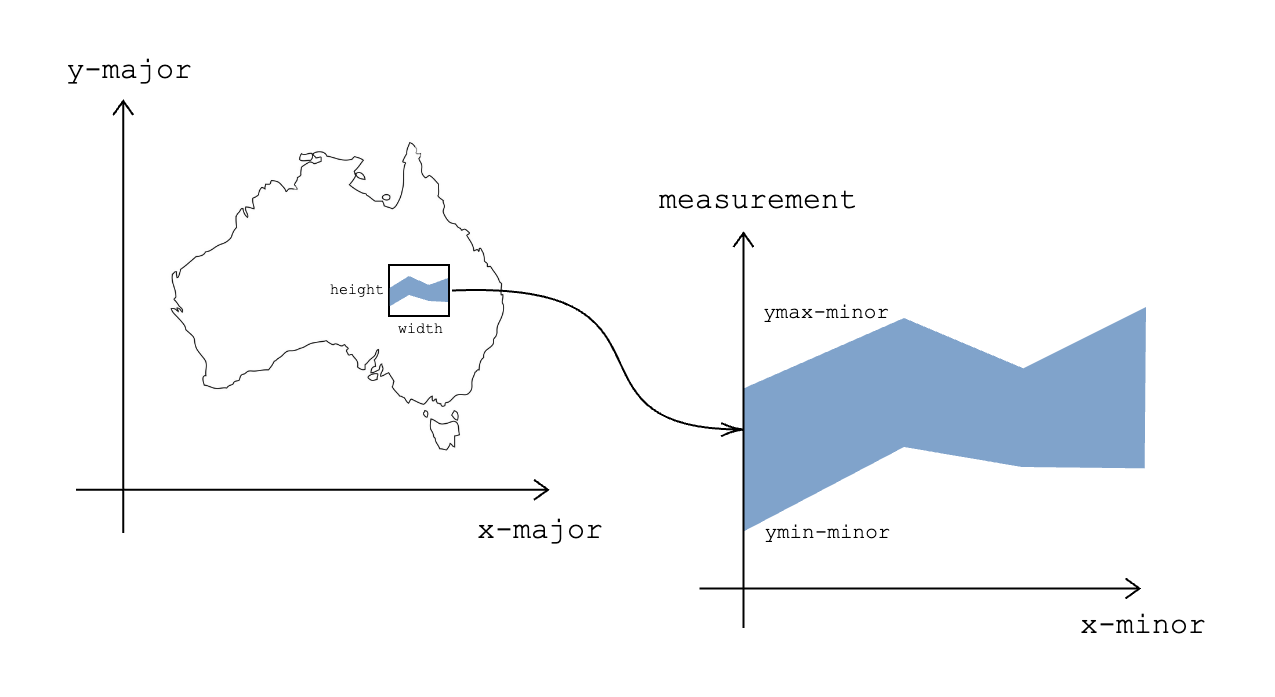
\includegraphics[width=17.71in]{figures/diagram-transformation} \caption{Diagram highlights how spatial data (geographical location) is combined with temporal data (measurements over time) to create a spatio-temporal visualization. In sugarglider, the transformation maps each station's temporal measurements into a visual glyph, allowing users to see patterns over time across different spatial locations.}\label{fig:unnamed-chunk-6}
\end{figure}

The construction of a glyph map, as described in Wickham et al. (2012), involves a linear combination of two key structural components: spatial location and data values. In this context, the major axes represent the spatial coordinates, latitude (\(y_{major}\)) and longitude (\(x_{major}\)), while the minor axes correspond to time (\(x_{minor}\)) and a measurement of interest (\(ymax_{minor}\) and \(ymin_{minor}\)). For segment glyphs, the measurement is represented by \(y_{minor}\) and \(yend_{minor}\).

Once the minor axes are rescaled to the interval {[}-1, 1{]}, the final coordinates for the ribbon glyph are determined through a linear transformation, as follows:

\[
x = x_{major} + \frac{width}{2} \cdot x_{minor}
\]

\[
ymin = y_{major} + \frac{height}{2} \cdot ymin_{minor}
\]

\[
ymax = y_{major} + \frac{height}{2} \cdot ymax_{minor}
\]

Similarly, the coordinates for the segment glyph are computed as:

\[
x = x_{major} + \frac{width}{2} \cdot x_{minor}
\]

\[
y = y_{major} + \frac{height}{2} \cdot y_{minor}
\]

\[
yend = y_{major} + \frac{height}{2} \cdot yend_{minor}
\]

This linear transformation ensures that the temporal and data components are properly aligned with the spatial coordinates, enabling a clear and accurate visualization of spatio-temporal data.

\hypertarget{examples}{%
\subsubsection{Examples}\label{examples}}

The \texttt{aus\_temp} dataset is used to demonstrate the functionality of the sugarglider package. Using the default rescaling parameters, we can visualize temperature data with \texttt{geom\_glyph\_segment()}, alongside \texttt{geom\_point()} that mark the location of each weather station. Each segment glyph represents local climate data, providing an intuitive way to explore temperature variations across Australia.

The default identity scaling function is applied to each set of minor values within each glyph. This method centers the glyphs both vertically and horizontally based on the station's coordinates and adjusts the minor axes to fit within the interval {[}-1, 1{]}. This ensures that the glyphs are appropriately scaled and sized to fit within the defined dimensions of the glyph.

\begin{verbatim}
aus_temp |>
  ggplot(aes(
    x_major = long, 
    y_major = lat, 
    x_minor = month, 
    y_minor = tmin, 
    yend_minor = tmax)) +
  add_glyph_boxes() +
  geom_point(aes(x = long, y = lat,
                 color = "Weather Station")) +
  geom_glyph_segment() +
  theme_glyph()
\end{verbatim}

\begin{figure}
\centering
\includegraphics{sugarglider_files/figure-latex/unnamed-chunk-8-1.pdf}
\caption{\label{fig:unnamed-chunk-8}Additional codes are needed for base map}
\end{figure}

The previous segment glyph map used global rescaling (enabled by default), meaning the glyphs were sized relative to one another based on their data values. By disabling global rescaling, we can observe the effects of local rescaling, where each glyph is resized according to its individual values.

\begin{itemize}
\tightlist
\item
  Local Rescale (global\_rescale = FALSE): Each line segment's length is determined by the local temperature range within a region, highlighting regional differences in temperature patterns.
\item
  Global Rescale (global\_rescale = TRUE): The global temperature range dictates the length of each line segment, ensuring consistent data scaling across all regions, which facilitates easy comparison.
\end{itemize}

Building on the analysis, precipitation data across Australia can be visualized using \texttt{geom\_glyph\_ribbon()}. The glyphs are color-coded to represent different levels of rainfall, while reference lines and glyph boxes are added to improve clarity and facilitate easy comparisons of precipitation levels across the country.

\begin{verbatim}
aus_temp |>
   group_by(id) |>
   mutate(prcp = mean(prcp, na.rm = TRUE)) |>
   ggplot(aes(x_major = long, y_major = lat,
              x_minor = month, ymin_minor = tmin,
              ymax_minor = tmax, 
              fill = prcp, color = prcp)) +
   add_glyph_boxes() +
   add_ref_lines() +
   geom_glyph_ribbon() +
   theme_glyph()
\end{verbatim}

\begin{figure}
\centering
\includegraphics{sugarglider_files/figure-latex/unnamed-chunk-10-1.pdf}
\caption{\label{fig:unnamed-chunk-10}Additional codes are needed for base map, and additonal theme customisation}
\end{figure}

To compare temperature trends across different years for specific regions in Victoria, \texttt{geom\_glyph\_ribbon()} offers an effective way to visualize how temperatures have evolved over time. Each year is distinguished by a different color, making the trends clear and easy to interpret.

\begin{verbatim}
historical_temp |> 
  filter(id %in% c("ASN00026021", "ASN00085291", "ASN00084143")) |>
   ggplot(aes(color = factor(year), fill = factor(year),
              group = interaction(year,id),
              x_major = long, y_major = lat,
              x_minor = month, ymin_minor = tmin, 
              ymax_minor = tmax)) +
   add_glyph_boxes() +
   add_ref_lines() +
   geom_glyph_ribbon() +
   theme_glyph()
\end{verbatim}

\begin{figure}
\centering
\includegraphics{sugarglider_files/figure-latex/unnamed-chunk-12-1.pdf}
\caption{\label{fig:unnamed-chunk-12}Additonal codes are needed for base map, title and additonal theme customisation}
\end{figure}

To further improve map readability, the \texttt{add\_geom\_legend()} function integrates an enlarged version of one of the glyphs in the bottom left corner of the plot. This legend helps users interpret the data scale more effectively.

In the example below, ribbon glyph-map is created using geom\_glyph\_ribbon() and overlaid on a basemap to depict daily temperature variations across Australian weather stations. A legend is added via \texttt{add\_glyph\_legend()}, allowing users to easily interpret the range of daily temperature values based on a randomly selected weather station. Since the legend data is drawn from a single, randomly chosen station, it is important to set a seed for reproducibility to ensure consistent results.

\begin{verbatim}
set.seed(28493)
aus_temp |>
   ggplot(aes(x_major = long, y_major = lat,
              x_minor = month, ymin_minor = tmin,
              ymax_minor = tmax)) +
  add_glyph_boxes() +
  add_ref_lines() +
  add_glyph_legend() +
  geom_glyph_ribbon() +
  theme_glyph() 
\end{verbatim}

\begin{figure}
\centering
\includegraphics{sugarglider_files/figure-latex/unnamed-chunk-14-1.pdf}
\caption{\label{fig:unnamed-chunk-14}Additonal code are needed for base map and additional theme customisation}
\end{figure}

In the following example, flight data is used to demonstrate the interactive glyph map capabilities of sugarglider. The U.S. Department of Transportation (DOT) Bureau of Transportation Statistics, which monitors the on-time performance of domestic flights operated by major U.S. airlines. Each month, the DOT publishes the Air Travel Consumer Report, summarizing on-time, delayed, canceled, and diverted flights.

This dataset, sourced from the Kaggle Airline Flight Delay and Cancellation data, has been processed and aggregated to display the minimum and maximum number of flights originating from the top 10 U.S. airports with the highest cancellation rates.

\begin{table}
\centering
\begin{tabular}{l|r|r|r|r|r}
\hline
origin & month & long & lat & min\_flights & max\_flights\\
\hline
ATL & 1 & -84.42806 & 33.63667 & 2321 & 3279\\
\hline
ATL & 2 & -84.42806 & 33.63667 & 1953 & 3074\\
\hline
ATL & 3 & -84.42806 & 33.63667 & 2667 & 3476\\
\hline
ATL & 4 & -84.42806 & 33.63667 & 896 & 3361\\
\hline
ATL & 5 & -84.42806 & 33.63667 & 785 & 3441\\
\hline
ATL & 6 & -84.42806 & 33.63667 & 1119 & 3473\\
\hline
\end{tabular}
\end{table}

This example showcases the functionality of \texttt{geom\_glyph\_segment()}, displaying the monthly range of flights for each airport and offering insights into how flight numbers fluctuate over time. Additionally, \texttt{geom\_glyph\_ribbon()} is used to visualize the variation between the minimum and maximum number of flights from each airport, providing a clear depiction of the spread in flight activity.

\begin{verbatim}
# Specify tooltip for ggiraph 
flights <- flights |>
  mutate(tooltip = paste("origin: ",origin,
                         "\nmonth: ", month,
                         "\nmin_flights: ", min_flights,
                         "\nmax_flights: ", max_flights))

fl <- flights |> 
  ggplot(aes(x_major = long, y_major = lat,
             x_minor = month, y_minor = min_flights,
             yend_minor = max_flights,
             tooltip = tooltip)) + 
  add_glyph_boxes() +
  add_ref_lines() +
  geom_glyph_segment() +
  theme_glyph()

# Interactive plot using ggiraph
# girafe(ggobj = fl)
\end{verbatim}

This plot displays the minimum and maximum number of flights departing from each airport on a spatial map. Each line segment represents the flight range for a respective airport, with the length of the segment indicating variability in flight numbers across different locations. Notably, airports like ATL and ORD typically handle a higher volume of departing flights compared to airports such as MCO and PHX. Additionally, all airports show fluctuations throughout the year, with wider flight intervals mid-year and narrower intervals during the holiday season at year-end.

The graph highlights that airports in certain regions experience more variability than others. While the segment plots provide a clear estimation of this variability, geom\_glyph\_ribbon() enhances understanding by visually representing the gap between the minimum and maximum flights. Wider ribbons suggest greater month-to-month fluctuations in flight operations.

\begin{verbatim}
# South Region
flights |> 
  filter(origin %in% c("ATL", "CLT", "MCO", "DFW")) |>
  ggplot(aes(x_major = long, y_major = lat,
             x_minor = month, ymin_minor = min_flights,
             ymax_minor = max_flights)) + 
  add_glyph_boxes() +
  add_ref_lines() +
  geom_glyph_ribbon() +
  theme_glyph()

# West region
flights |> 
  filter(origin %in% c("PHX", "LAS", "LAX", "SEA")) |>
  ggplot(aes(x_major = long, y_major = lat,
             x_minor = month, ymin_minor = min_flights,
             ymax_minor = max_flights)) + 
  add_glyph_boxes() +
  add_ref_lines() +
  geom_glyph_ribbon() +
  theme_glyph()
\end{verbatim}

\begin{figure}
\centering
\includegraphics{sugarglider_files/figure-latex/unnamed-chunk-19-1.pdf}
\caption{\label{fig:unnamed-chunk-19}Additonal code are needed for base map and additional theme customisation}
\end{figure}

\texttt{geom\_glyph\_ribbon()} effectively highlights the disparities in flight volume between regions. The Western region exhibits a greater variation in the number of flights compared to the Southern region, as evidenced by the thicker ribbons. Notably, both regions display a significant increase in flight volume discrepancies during the mid-year, reinforcing the findings observed with \texttt{geom\_glyph\_segment()}.

\hypertarget{application}{%
\section{Application}\label{application}}

Five examples are selected to demonstrate various features of the sugarglider package: (1) Creating a ribbon glyph map to visualize annual fluctuations in minimum and maximum daily patronage for each train station, revealing seasonal trends. (2) Using glyph segments to compare patronage on typical weekdays versus weekends at different stations, enabling insights for optimizing service schedules. (3) Utilizing glyph ribbons to represent variations in patronage during distinct peak periods---AM peak, interpeak, PM peak, and late PM hours---across stations. (4) Displaying differences in patronage across transportation modes (Metro, VLine, or both) using glyph segments, identifying capacity imbalances. Lastly, (5) Employing glyph ribbons to compare public and school holiday patronage against regular days, aiding in scheduling and resource planning.

\hypertarget{yearly-patronage-changes-by-station}{%
\subsubsection{Yearly Patronage Changes by Station}\label{yearly-patronage-changes-by-station}}

\hypertarget{weekday-vs.-weekend-patronage}{%
\subsubsection{Weekday vs.~Weekend Patronage}\label{weekday-vs.-weekend-patronage}}

\hypertarget{patronage-during-different-peak-times}{%
\subsubsection{Patronage During Different Peak Times}\label{patronage-during-different-peak-times}}

\hypertarget{patronage-variations-by-transportation-mode}{%
\subsubsection{Patronage Variations by Transportation Mode}\label{patronage-variations-by-transportation-mode}}

\hypertarget{public-and-school-holiday-patronage-vs.-regular-days}{%
\subsubsection{Public and School Holiday Patronage vs.~Regular Days}\label{public-and-school-holiday-patronage-vs.-regular-days}}

\hypertarget{discussion}{%
\section{Discussion}\label{discussion}}

\hypertarget{acknowledgements}{%
\section{Acknowledgements}\label{acknowledgements}}

\hypertarget{references}{%
\section*{References}\label{references}}
\addcontentsline{toc}{section}{References}

\hypertarget{refs}{}
\begin{CSLReferences}{1}{0}
\leavevmode\vadjust pre{\hypertarget{ref-wickham2012glyph}{}}%
Wickham, Hadley, Heike Hofmann, Charlotte Wickham, and Dianne Cook. 2012. {``Glyph-Maps for Visually Exploring Temporal Patterns in Climate Data and Models.''} \emph{Environmetrics} 23 (5): 382--93.

\leavevmode\vadjust pre{\hypertarget{ref-JSSv110i07}{}}%
Zhang, H. Sherry, Dianne Cook, Ursula Laa, Nicolas Langrené, and Patricia Menéndez. 2024. {``Cubble: An r Package for Organizing and Wrangling Multivariate Spatio-Temporal Data.''} \emph{Journal of Statistical Software} 110 (7): 1--27. \url{https://doi.org/10.18637/jss.v110.i07}.

\end{CSLReferences}


\address{%
Maliny Po\\
Monash University\\%
Department of Econometrics and Business Statistics\\ Melbourne, Australia\\
%
%
\textit{ORCiD: \href{https://orcid.org/0009-0008-4686-6631}{0009-0008-4686-6631}}\\%
\href{mailto:malinypo12@gmail.com}{\nolinkurl{malinypo12@gmail.com}}%
}

\address{%
Dianne Cook\\
Monash University\\%
Department of Econometrics and Business Statistics\\ Melbourne, Australia\\
%
%
\textit{ORCiD: \href{https://orcid.org/0000-0002-3813-7155}{0000-0002-3813-7155}}\\%
\href{mailto:dicook@monash.edu}{\nolinkurl{dicook@monash.edu}}%
}

\end{article}


\end{document}
